\subsection{Crear una partida}

\begin{figure}[ht]
\centering
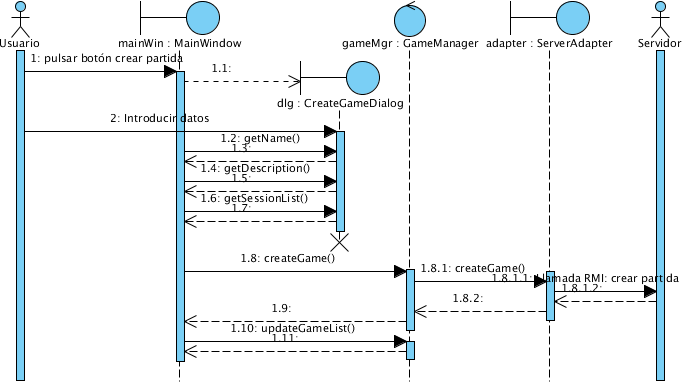
\includegraphics[scale=0.6]{img/ch03devel-creategame.png}
\caption{Diagrama de secuencia de ``Crear una partida''}
\end{figure}

Cuando el usuario seleccione la opción de crear una nueva partida, se le
mostrará una ventana diálogo donde podrá seleccionar los parámetros de esta
nueva partida.

Con estos datos, la ventana principal solicitará al gestor de partidas la
creación de una nueva partida. Si no ocurre ninguna excepción, se realizará una
llamada al caso de uso anterior, actualizar lista de partidas, para que se
actualicen los modelos de datos, y por tanto la interfaz de usuario.
